\documentclass[tikz,border=10pt]{standalone}
\usepackage{tikz}
\usetikzlibrary{shapes.geometric, shapes.multipart, arrows.meta, positioning, calc, fit, backgrounds, shadows, patterns}

% Define colors to match main document
\definecolor{blue}{RGB}{0,0,255}
\definecolor{orange}{RGB}{255,165,0}
\definecolor{dkgreen}{RGB}{0,100,0}
\definecolor{gray}{RGB}{128,128,128}
\definecolor{darkgray}{RGB}{64,64,64}

\begin{document}
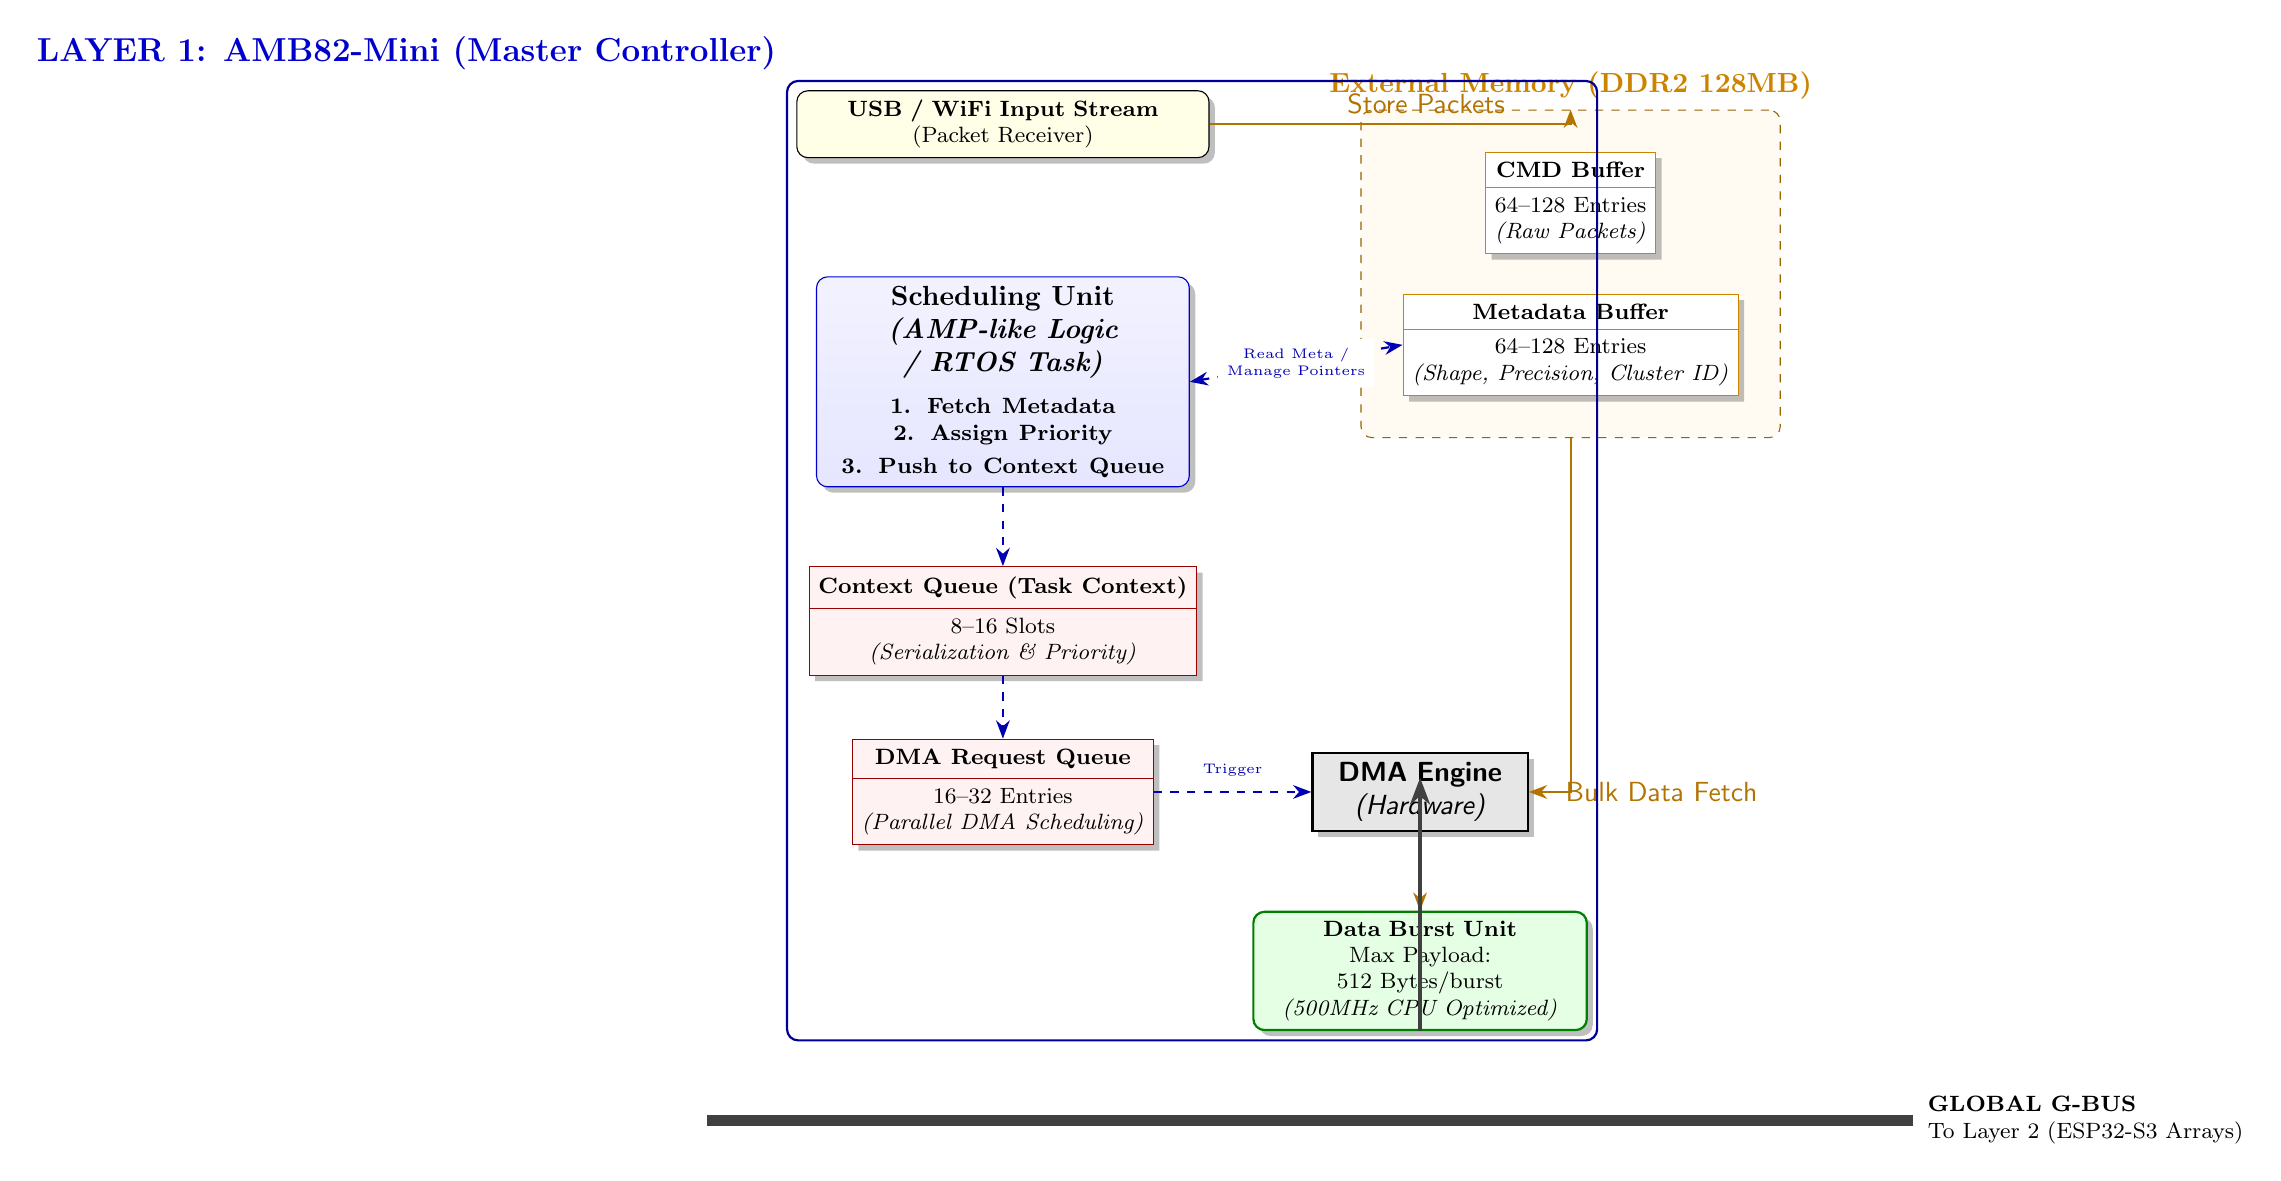
\begin{tikzpicture}[
    font=\sffamily,
    % 樣式定義
    component/.style={
        draw, fill=white, rounded corners, align=center, drop shadow, font=\footnotesize
    },
    scheduler_block/.style={
        draw=blue!80!black, top color=blue!5, bottom color=blue!10, 
        rounded corners, align=center, drop shadow, font=\bfseries
    },
    memory_container/.style={
        draw=orange!60!black, fill=orange!5, dashed, rounded corners, inner sep=15pt,
        label={[orange!80!black, font=\bfseries]north:External Memory (DDR2 128MB)}
    },
    buffer_block/.style={
        draw=orange!80!black, fill=white, rectangle split, rectangle split parts=2, 
        align=center, drop shadow, font=\footnotesize
    },
    queue_block/.style={
        draw=red!60!black, fill=red!5, rectangle split, rectangle split parts=2,
        align=center, drop shadow, font=\footnotesize, minimum width=3.5cm
    },
    dma_block/.style={
        draw=black, fill=gray!20, thick, align=center, drop shadow
    },
    bus/.style={
        draw=darkgray, line width=4pt
    },
    bus_arrow/.style={
        ->, >=Stealth, thick, color=darkgray, line width=1.5pt
    },
    control_flow/.style={
        ->, >=Stealth, dashed, blue!70!black, thick
    },
    data_flow/.style={
        ->, >=Stealth, thick, orange!70!black
    }
]

    % --- 1. TOP INTERFACE (Host Input) ---
    \node[component, fill=yellow!10, text width=5cm] (host_io) at (0, 0) {
        \textbf{USB / WiFi Input Stream}\\
        (Packet Receiver)
    };

    % --- 2. DDR2 MEMORY BLOCK (Right Side) ---
    % Increased spacing from 2cm to 3.5cm to prevent overlap
    \node[buffer_block, right=3.5cm of host_io, yshift=-1cm] (ddr_buffers) {
        \textbf{CMD Buffer}
        \nodepart{second} 64--128 Entries\\
        \textit{(Raw Packets)}
    };
    
    \node[buffer_block, below=0.5cm of ddr_buffers] (meta_buffers) {
        \textbf{Metadata Buffer}
        \nodepart{second} 64--128 Entries\\
        \textit{(Shape, Precision, Cluster ID)}
    };

    \begin{scope}[on background layer]
        % Removed explicit label to avoid duplication with style definition
        \node[memory_container, fit=(ddr_buffers) (meta_buffers)] (ddr_frame) {};
    \end{scope}

    % Connect Host to DDR
    \draw[data_flow] (host_io.east) -| (ddr_frame.north) node[pos=0.3, above] {Store Packets};

    % --- 3. AMP SCHEDULER (Center) ---
    \node[scheduler_block, below=1.5cm of host_io, text width=4.5cm, minimum height=2cm] (scheduler) {
        \textbf{Scheduling Unit}\\
        \textit{(AMP-like Logic / RTOS Task)}\\
        \vspace{0.2cm}
        \footnotesize
        1. Fetch Metadata\\
        2. Assign Priority\\
        3. Push to Context Queue
    };

    % Interaction: Scheduler reads DDR
    \draw[control_flow, <->] (scheduler.east) -- node[midway, fill=white, font=\tiny, align=center] {Read Meta /\\Manage Pointers} (meta_buffers.west);

    % --- 4. QUEUING SYSTEM (Below Scheduler) ---
    
    % Context Queue
    \node[queue_block, below=1cm of scheduler] (ctx_queue) {
        \textbf{Context Queue (Task Context)}
        \nodepart{second} 8--16 Slots\\
        \textit{(Serialization \& Priority)}
    };

    % DMA Request Queue
    \node[queue_block, below=0.8cm of ctx_queue] (dma_queue) {
        \textbf{DMA Request Queue}
        \nodepart{second} 16--32 Entries\\
        \textit{(Parallel DMA Scheduling)}
    };

    % Flow: Scheduler -> Ctx -> DMA
    \draw[control_flow] (scheduler.south) -- (ctx_queue.north);
    \draw[control_flow] (ctx_queue.south) -- (dma_queue.north);

    % --- 5. EXECUTION ENGINE (Bottom) ---
    
    % DMA Engine
    % Align clearly to the right
    \node[dma_block, right=2.0cm of dma_queue, text width=2.5cm] (dma_engine) {
        \textbf{DMA Engine}\\
        \textit{(Hardware)}
    };

    % Data Burst Unit
    \node[component, below=1cm of dma_engine, text width=4cm, fill=green!10, draw=green!50!black, thick] (burst_unit) {
        \textbf{Data Burst Unit}\\
        Max Payload: 512 Bytes/burst\\
        \textit{(500MHz CPU Optimized)}
    };

    % Connecting Memory Data to Output via DMA
    % Rerouted to enter from NORTH for cleaner vertical flow
    \draw[data_flow] (ddr_frame.south) |- (dma_engine.east) node[near end, right, xshift=2pt] {Bulk Data Fetch};
    \draw[control_flow] (dma_queue.east) -- (dma_engine.west) node[midway, above, font=\tiny, yshift=2pt] {Trigger};
    \draw[data_flow] (dma_engine.south) -- (burst_unit.north);

    % --- 6. LAYER FRAME ---
    \node[draw=blue!60!black, thick, rounded corners, fit=(host_io) (scheduler) (burst_unit) (dma_queue), label={[blue!80!black, font=\large\bfseries]north west:LAYER 1: AMB82-Mini (Master Controller)}] (layer1_frame) {};

    % --- 7. GLOBAL BUS INTERFACE ---
    \draw[bus] ($(layer1_frame.south west) + (-1, -1)$) -- ($(layer1_frame.south east) + (4, -1)$) node[right, align=left, font=\footnotesize] {
        \textbf{GLOBAL G-BUS}\\
        To Layer 2 (ESP32-S3 Arrays)
    };

    \draw[bus_arrow] (burst_unit.south) -- (burst_unit.south |- layer1_frame.south |- 0, -8.3);

\end{tikzpicture}
\end{document}
